% zReg library class diagram — src/zreg (feature/evaluation_framework)
% Compile with:  pdflatex zreg_class_diagram.tex
%
% Layout (left → right follows the pipeline):
%
%  ┌─────────────────── core (foundation) ────────────────────────────────┐
%  └──────────────────────────────────────────────────────────────────────┘
%   data_generation → preprocessing →  algorithms  → label_transfer → evaluation
%                                      [cpd] [dtw]
%                                      ↑              ↑
%                               distance_metrics    models
%
\documentclass{article}
\usepackage[a3paper, landscape, top=0.8cm, bottom=0.8cm,
            left=0.8cm, right=0.8cm]{geometry}
\usepackage{lmodern}
\usepackage[T1]{fontenc}
\usepackage{tikz}
\usetikzlibrary{arrows.meta, backgrounds, fit, calc}
\usepackage{xcolor}
\pagestyle{empty}
\setlength\parindent{0pt}

%% Colour scheme: one hue (steel-blue), two intensities
%% - all top-level modules: MOD (medium blue tint)
%% - submodules nested inside a module: SUB (lighter tint)
\definecolor{MOD}{RGB}{210,224,240}   % module background
\definecolor{SUB}{RGB}{232,241,251}   % submodule background
\definecolor{BD}{RGB}{60,78,96}       % border / text

\tikzset{
  %% Class boxes (white fill, uniform border)
  cls/.style={
    rectangle, draw=BD!70, fill=white,
    minimum width=3.0cm, minimum height=0.64cm,
    align=center, font=\scriptsize\sffamily,
    rounded corners=1pt, inner sep=3pt
  },
  abscls/.style={cls, font=\scriptsize\sffamily\itshape},
  %% Function-list module box
  fbox/.style={
    rectangle, draw=BD!70, fill=white,
    align=left, font=\scriptsize\sffamily,
    rounded corners=1pt, inner sep=5pt,
    text width=3.6cm
  },
  %% Package containers
  pkgbox/.style={
    rectangle, draw=BD!50, fill=MOD,
    rounded corners=3pt, inner sep=7pt,
    line width=0.65pt
  },
  subbox/.style={
    rectangle, draw=BD!40, fill=SUB,
    rounded corners=2pt, inner sep=6pt,
    line width=0.5pt
  },
  pkglbl/.style={font=\footnotesize\sffamily\bfseries, text=BD},
  sublbl/.style={font=\scriptsize\sffamily\bfseries, text=BD!80},
  stlbl/.style={font=\tiny\sffamily\itshape, text=BD!55},
  %% Arrows
  inh/.style={   % generalisation — open hollow triangle at parent end
    -{Triangle[open,length=5pt,width=5pt]},
    line width=0.8pt, color=BD
  },
  impl/.style={  % realisation (Protocol) — dashed
    dashed, -{Triangle[open,length=5pt,width=5pt]},
    line width=0.75pt, color=BD
  },
  uses/.style={  % dependency / uses
    -latex, dashed, line width=0.5pt, color=BD!60
  },
  prod/.style={  % produces / returns
    -latex, line width=0.55pt, color=BD!55
  },
  aggr/.style={  % aggregation — open diamond at container end
    {Diamond[open,length=4.5pt,width=4pt]}-,
    line width=0.6pt, color=BD!60
  },
  pipe/.style={  % pipeline data-flow arrow
    -latex, line width=1.1pt, color=BD!65
  },
}

\begin{document}\noindent
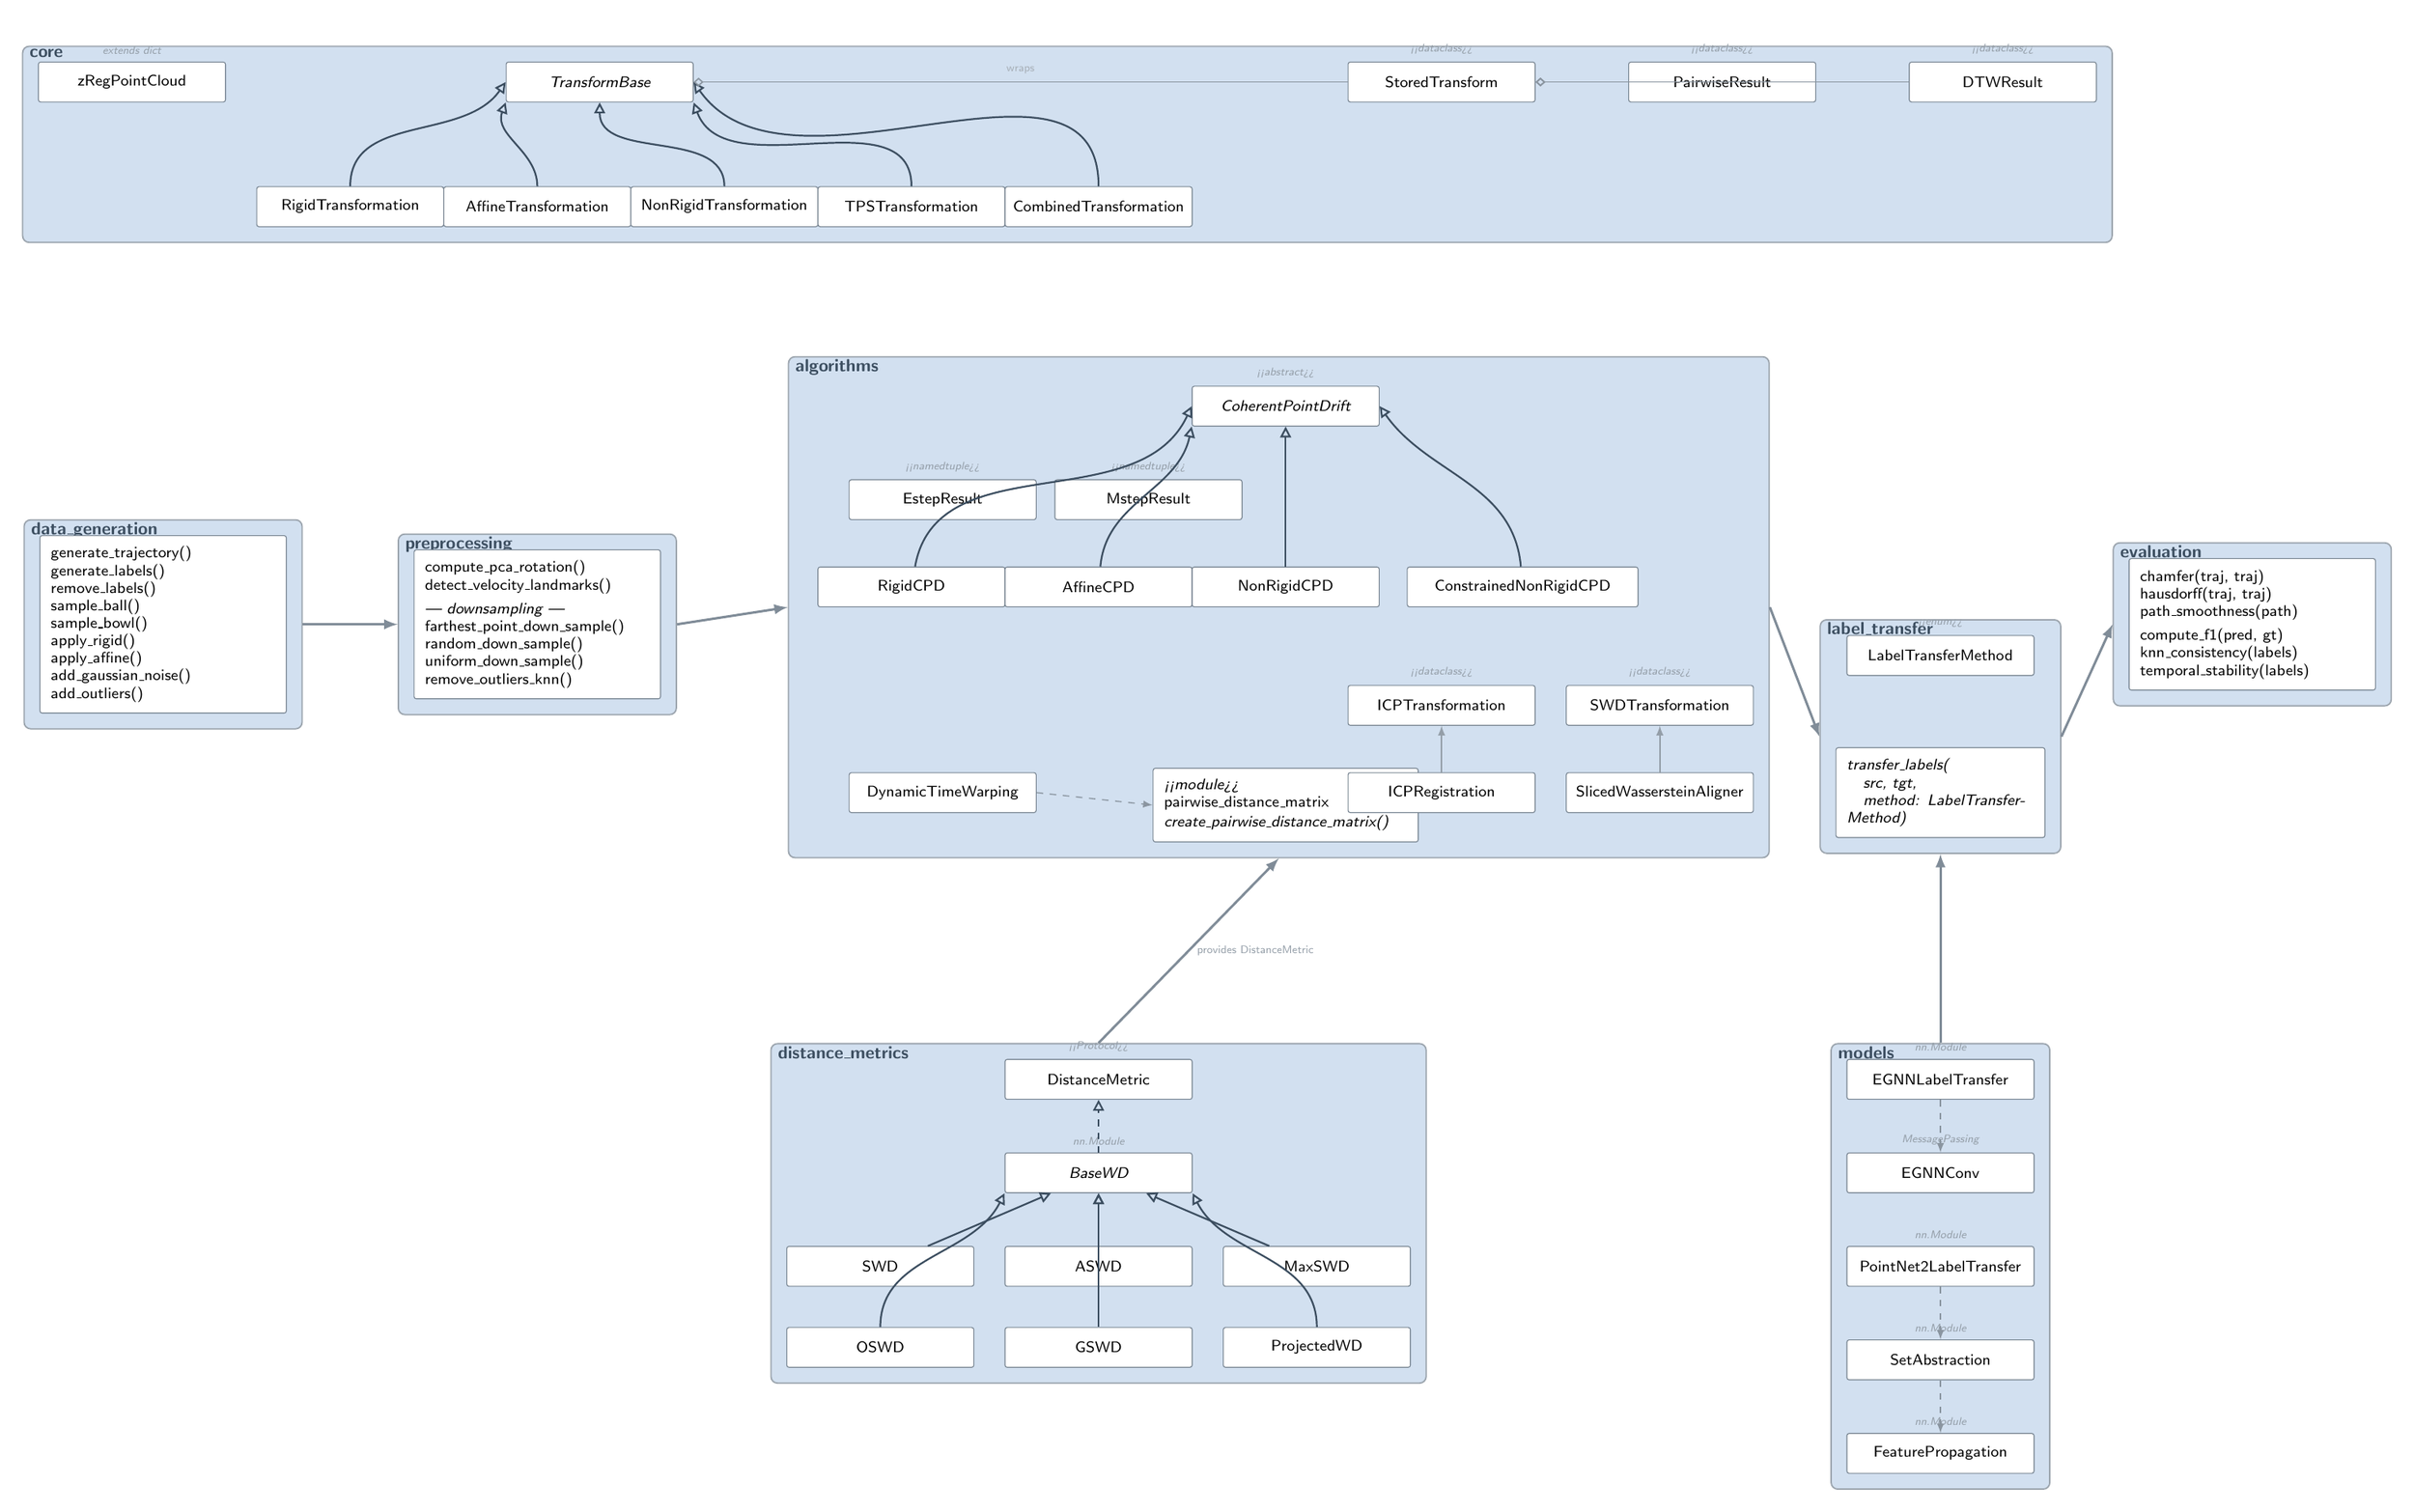
\begin{tikzpicture}[x=1cm, y=1cm]

%% ================================================================
%%  CORE  (top strip, y = 23.5 … 28)
%% ================================================================

\node[cls, label={[stlbl]above:extends dict}]
  (zregpc)    at ( 2.0, 27.2) {zRegPointCloud};
\node[abscls]
  (transbase) at ( 9.5, 27.2) {TransformBase};

\node[cls] (rigid)   at ( 5.5, 25.2) {RigidTransformation};
\node[cls] (affine)  at ( 8.5, 25.2) {AffineTransformation};
\node[cls] (nrigd)   at (11.5, 25.2) {NonRigidTransformation};
\node[cls] (tps)     at (14.5, 25.2) {TPSTransformation};
\node[cls] (comb)    at (17.5, 25.2) {CombinedTransformation};

\node[cls, label={[stlbl]above:<<dataclass>>}]
  (storedtf)  at (23.0, 27.2) {StoredTransform};
\node[cls, label={[stlbl]above:<<dataclass>>}]
  (pairwiser) at (27.5, 27.2) {PairwiseResult};
\node[cls, label={[stlbl]above:<<dataclass>>}]
  (dtwresult) at (32.0, 27.2) {DTWResult};

%% Inheritance fan into TransformBase
\draw[inh] (rigid.north)  to[out=90,in=235] (transbase.west);
\draw[inh] (affine.north) to[out=90,in=250] (transbase.south west);
\draw[inh] (nrigd.north)  to[out=90,in=270] (transbase.south);
\draw[inh] (tps.north)    to[out=90,in=290] (transbase.south east);
\draw[inh] (comb.north)   to[out=90,in=305] (transbase.east);

%% StoredTransform wraps a TransformBase; aggregated by PairwiseResult + DTWResult
\draw[aggr] (transbase.east)
  -- node[above,font=\tiny\sffamily,text=BD!45]{wraps}
  (storedtf.west);
\draw[aggr] (storedtf.east)   -- (pairwiser.west);
\draw[aggr] (storedtf.east) to[out=0,in=180] (dtwresult.west);

\begin{pgfonlayer}{background}
  \node[pkgbox,
    fit=(zregpc)(transbase)(rigid)(affine)(nrigd)(tps)(comb)
        (storedtf)(pairwiser)(dtwresult)]
    (corebox) {};
  \node[pkglbl, anchor=north west, yshift=2pt] at (corebox.north west) {core};
\end{pgfonlayer}

%% ================================================================
%%  PIPELINE ROW (y ≈ 13.5 … 23)
%% ================================================================

%%--- data_generation (leftmost) ---
\node[fbox] (datagmod) at (2.5, 18.5)
  {generate\_trajectory()\\
   generate\_labels()\\
   remove\_labels()\\
   sample\_ball()\\
   sample\_bowl()\\
   apply\_rigid()\\
   apply\_affine()\\
   add\_gaussian\_noise()\\
   add\_outliers()};

\begin{pgfonlayer}{background}
  \node[pkgbox, fit=(datagmod)] (datagbox) {};
  \node[pkglbl, anchor=north west, yshift=2pt]
    at (datagbox.north west) {data\_generation};
\end{pgfonlayer}

%%--- preprocessing ---
\node[fbox] (premod) at (8.5, 18.5)
  {compute\_pca\_rotation()\\
   detect\_velocity\_landmarks()\\[3pt]
   \textit{--- downsampling ---}\\
   farthest\_point\_down\_sample()\\
   random\_down\_sample()\\
   uniform\_down\_sample()\\
   remove\_outliers\_knn()};

\begin{pgfonlayer}{background}
  \node[pkgbox, fit=(premod)] (prebox) {};
  \node[pkglbl, anchor=north west, yshift=2pt]
    at (prebox.north west) {preprocessing};
\end{pgfonlayer}

%%--- algorithms (widest — contains cpd and dtw subpackages) ---

% algorithms / cpd subpackage
\node[abscls, label={[stlbl]above:<<abstract>>}]
  (cpd) at (20.5, 22.0) {CoherentPointDrift};

\node[cls, label={[stlbl]above:<<namedtuple>>}]
  (estep) at (15.0, 20.5) {EstepResult};
\node[cls, label={[stlbl]above:<<namedtuple>>}]
  (mstep) at (18.3, 20.5) {MstepResult};

\node[cls] (rigcpd)  at (14.5, 19.1) {RigidCPD};
\node[cls] (affcpd)  at (17.5, 19.1) {AffineCPD};
\node[cls] (nrigcpd) at (20.5, 19.1) {NonRigidCPD};
\node[cls, minimum width=3.7cm]
  (cnrcpd) at (24.3, 19.1) {ConstrainedNonRigidCPD};

\draw[inh] (rigcpd)  to[out=80,in=245] (cpd.west);
\draw[inh] (affcpd)  to[out=85,in=258] (cpd.south west);
\draw[inh] (nrigcpd) --               (cpd);
\draw[inh] (cnrcpd)  to[out=95,in=305] (cpd.east);

\begin{pgfonlayer}{background}
  \node[subbox,
    fit=(cpd)(estep)(mstep)(rigcpd)(affcpd)(nrigcpd)(cnrcpd)]
    (cpdbox) {};
  \node[sublbl, anchor=north west, yshift=2pt]
    at (cpdbox.north west) {cpd};
\end{pgfonlayer}

% algorithms / dtw subpackage
\node[cls] (dtw) at (15.0, 15.8) {DynamicTimeWarping};

\begin{pgfonlayer}{background}
  \node[subbox, fit=(dtw)] (dtwbox) {};
  \node[sublbl, anchor=north west, yshift=2pt]
    at (dtwbox.north west) {dtw};
\end{pgfonlayer}

% pairwise_distance_matrix module (flat file in algorithms/)
\node[fbox, text width=3.9cm] (pdm) at (20.5, 15.6)
  {\textit{<<module>>}\\
   pairwise\_distance\_matrix\\[1pt]
   \textit{create\_pairwise\_distance\_matrix()}};

% ICP
\node[cls, label={[stlbl]above:<<dataclass>>}]
  (icptf)  at (23.0, 17.2) {ICPTransformation};
\node[cls] (icpreg) at (23.0, 15.8) {ICPRegistration};

% SWD Aligner
\node[cls, label={[stlbl]above:<<dataclass>>}]
  (swdtf)  at (26.5, 17.2) {SWDTransformation};
\node[cls] (swdalg) at (26.5, 15.8) {SlicedWassersteinAligner};

\draw[prod] (icpreg.north) -- (icptf.south);
\draw[prod] (swdalg.north) -- (swdtf.south);
\draw[uses] (dtw.east) -- (pdm.west);

\begin{pgfonlayer}{background}
  \node[pkgbox,
    fit=(cpdbox)(dtwbox)(pdm)(icptf)(icpreg)(swdtf)(swdalg)]
    (algobox) {};
  \node[pkglbl, anchor=north west, yshift=2pt]
    at (algobox.north west) {algorithms};
\end{pgfonlayer}

%%--- label_transfer ---
\node[cls, label={[stlbl]above:<<enum>>}]
  (ltmeth) at (31.0, 18.0) {LabelTransferMethod};
\node[fbox, text width=3.0cm] (ltfn) at (31.0, 15.8)
  {\textit{transfer\_labels(}\\
   \textit{\quad src, tgt,}\\
   \textit{\quad method: LabelTransferMethod)}};

\begin{pgfonlayer}{background}
  \node[pkgbox, fit=(ltmeth)(ltfn)] (ltbox) {};
  \node[pkglbl, anchor=north west, yshift=2pt]
    at (ltbox.north west) {label\_transfer};
\end{pgfonlayer}

%%--- evaluation (rightmost) ---
\node[fbox] (evalmod) at (36.0, 18.5)
  {chamfer(traj, traj)\\
   hausdorff(traj, traj)\\
   path\_smoothness(path)\\[3pt]
   compute\_f1(pred, gt)\\
   knn\_consistency(labels)\\
   temporal\_stability(labels)};

\begin{pgfonlayer}{background}
  \node[pkgbox, fit=(evalmod)] (evalbox) {};
  \node[pkglbl, anchor=north west, yshift=2pt]
    at (evalbox.north west) {evaluation};
\end{pgfonlayer}

%% ================================================================
%%  SUPPORT ROW (y ≈ 0 … 12.5)
%%  Placed directly below the modules they feed into.
%% ================================================================

%%--- distance_metrics (below algorithms) ---
\node[cls, label={[stlbl]above:<<Protocol>>}]
  (distmet) at (17.5, 11.2) {DistanceMetric};
\node[abscls, label={[stlbl]above:nn.Module}]
  (basewd)  at (17.5,  9.7) {BaseWD};

\node[cls] (swd)   at (14.0, 8.2) {SWD};
\node[cls] (aswd)  at (17.5, 8.2) {ASWD};
\node[cls] (maxwd) at (21.0, 8.2) {MaxSWD};
\node[cls] (oswd)  at (14.0, 6.9) {OSWD};
\node[cls] (gswd)  at (17.5, 6.9) {GSWD};
\node[cls] (pwd)   at (21.0, 6.9) {ProjectedWD};

\draw[impl] (basewd)  --               (distmet);
\draw[inh]  (swd)     --               (basewd);
\draw[inh]  (aswd)    --               (basewd);
\draw[inh]  (maxwd)   --               (basewd);
\draw[inh]  (oswd)  to[out=90,in=243]  (basewd.south west);
\draw[inh]  (gswd)    --               (basewd);
\draw[inh]  (pwd)   to[out=90,in=297]  (basewd.south east);

\begin{pgfonlayer}{background}
  \node[pkgbox,
    fit=(distmet)(basewd)(swd)(aswd)(maxwd)(oswd)(gswd)(pwd)]
    (distbox) {};
  \node[pkglbl, anchor=north west, yshift=2pt]
    at (distbox.north west) {distance\_metrics};
\end{pgfonlayer}

%%--- models (below label_transfer) ---
\node[cls, label={[stlbl]above:nn.Module}]
  (egnnlt)   at (31.0, 11.2) {EGNNLabelTransfer};
\node[cls, label={[stlbl]above:MessagePassing}]
  (egnnconv) at (31.0,  9.7) {EGNNConv};
\node[cls, label={[stlbl]above:nn.Module}]
  (pn2lt)    at (31.0,  8.2) {PointNet2LabelTransfer};
\node[cls, label={[stlbl]above:nn.Module}]
  (setabs)   at (31.0,  6.7) {SetAbstraction};
\node[cls, label={[stlbl]above:nn.Module}]
  (featprop) at (31.0,  5.2) {FeaturePropagation};

\draw[uses] (egnnlt.south)  -- (egnnconv.north);
\draw[uses] (pn2lt.south)   -- (setabs.north);
\draw[uses] (setabs.south)  -- (featprop.north);

\begin{pgfonlayer}{background}
  \node[pkgbox,
    fit=(egnnlt)(egnnconv)(pn2lt)(setabs)(featprop)]
    (modelbox) {};
  \node[pkglbl, anchor=north west, yshift=2pt]
    at (modelbox.north west) {models};
\end{pgfonlayer}

%% ================================================================
%%  CROSS-PACKAGE ARROWS  (all route through empty space only)
%% ================================================================

%% Pipeline data-flow (horizontal, between adjacent boxes)
\draw[pipe] (datagbox.east)  -- (prebox.west);
\draw[pipe] (prebox.east)    -- (algobox.west);
\draw[pipe] (algobox.east)   -- (ltbox.west);
\draw[pipe] (ltbox.east)     -- (evalbox.west);

%% distance_metrics feeds algorithms — vertical arrow from below
\draw[pipe] (distbox.north) --
  node[right, font=\tiny\sffamily, text=BD!55, pos=0.5]{provides DistanceMetric}
  (algobox.south);

%% models feeds label_transfer — vertical arrow from below
\draw[pipe] (modelbox.north) -- (ltbox.south);

\end{tikzpicture}
\end{document}
